\documentclass[11pt, a4paper]{article}
\usepackage{graphicx, fullpage, hyperref, listings}
\usepackage{appendix, pdfpages, color}
\usepackage{indentfirst} %段首空两格 棒
\usepackage{chngpage} 
\usepackage{tocloft}            % This squashes the Table of Contents a bit
\usepackage{pdfpages}
\usepackage{multirow}
\usepackage{amsmath}
\usepackage{framed}


\setlength\cftbeforesecskip{3pt}
\renewcommand{\contentsname}{\centerline{\textbf{Content}}}
\graphicspath{{images/}}

\usepackage{multicol}

\usepackage{graphicx}
\usepackage{epstopdf}
\hypersetup{CJKbookmarks,%
	bookmarksnumbered,%
	colorlinks,%
	linkcolor=black,%
	citecolor=black,%
	plainpages=false,%
	pdfstartview=FitH}

%%%%%%%代码语法高亮设置

\usepackage{color}

\definecolor{pblue}{rgb}{0.13,0.13,1}
\definecolor{pgreen}{rgb}{0,0.5,0}
\definecolor{pred}{rgb}{0.9,0,0}
\definecolor{pgrey}{rgb}{0.46,0.45,0.48}

\usepackage{listings}
\lstset{
	language=Java,
	showspaces=false,
	showtabs=false,
	%%%%%
	frame = single,
	stepnumber = 2,  
	numbersep = 4pt, 
	 numbers=left,
	%breakatwhitespace=false, 
	tabsize=2,  
	%%%%%
	breaklines=true,
	showstringspaces=false,
    breakatwhitespace=false, 
	commentstyle=\color{pgreen},
	keywordstyle=\color{pblue},
	stringstyle=\color{pred},
	basicstyle=\ttfamily,
	%moredelim=[il][\textcolor{pgrey}]{$$},
	%moredelim=[is][\textcolor{pgrey}]{\%\%}{\%\%},
}


%%%%%%%%代码语法高亮设置

\definecolor{MyLightYellow}{cmyk}{0,0.,0.2,0} 

\setlength{\parskip}{4pt}        % sets spacing between paragraphs
\interfootnotelinepenalty=500    % this prevents footnotes breaking across pages

\title{\includegraphics[width=0.45\textwidth]{wpi2}
        \\CS 534 Artificial Intelligence \\ Assignment 2 }          % <<<<<<<<< change the title as appropriate
\author{Group 10 }                    % <<<<<<<<< module code

\begin{document}
\begin{titlepage}
	
%\date{\today}
\maketitle
\addtocontents{toc}{\protect\thispagestyle{empty}} % because we don't want a page number on the title page
% Thanks to Huang Shanyue for suggesting this 

\begin{center}
Group Member
\end{center}

\begin{table}[htbp] 
\begin{center}
\begin{tabular}{l l l} 
	 
	 Yixuan & Jiao  &   yjiao@wpi.edu \\
     Yinkai & Ma  &   yma7@wpi.edu \\
     Jiaming & Nie  &  jnie@wpi.edu \\
     Pinyi & Xiao  &  pxiao@wpi.edu \\
\end{tabular}
\end{center}
\end{table}



%\date{\today}
\thispagestyle{empty}  %去除首页页码

\end{titlepage}

%\tableofcontents
%\listoffigures

%\newpage



%\tableofcontents

%\listoffigures
%\listoftables
%\lstlistoflistings        


%\newpage

\section{Gibbs Sampling}



\section{Kalman Filter}

The transition model is constructed using the GDP and the gdp growth rate from 1970 to 2017, data source is from world bank website~\cite{ref:source1}. Unit is trillion dollar.

There are 2 sensor models, in the first model our group use the Export and Import data from 1970 to 2017~\cite{ref:source2}, the unit is value in million dollars, to measure the GDP only, which is use the 2 sensors to measure the GDP. 

The second model is use 3 sensors, the 2 sensors are still import and export, the additional sensor is the employment rate~\cite{ref:source3}, to measure the GDP growth rate. The data source is from Office of Management and Budget. 

\subsection{Methodology}

\subsubsection{Kalman Filter Graph Model and Equations}
The graph model of the Kalman filter is on the following:



The parameters of the Kalman filter and their equations are on the following~\cite{ref:kf}.

For Kalman filter, its parameters are listed in the table~\ref{tab:kf_meaning}:

\begin{table}[htbp] 
	\begin{center}
		\caption{Kalman Filter Parameters Notation}
		\begin{tabular}{|l|p{400pt}|} \hline
			Parameter & Notation \\ \hline
			${x_t}$ & The state vector containing the terms of interest for the system (e.g., position, velocity, heading) at a time 
			\\ \hline
			${F_t}$ & The state transition matrix which applies the effect of each system state at time \textit{t}. (e.g., the position and velocity at time t-1 both affect the position at time t) \\ \hline
			${w_t}$ & the vector which contains the noise for each parameter in the state vector ${x_t}$. A zero mean multivariate Gaussian distribution with covariance matrix ${Q_t}$ is used to describe the process noise vector. \\ \hline
			${z_t}$ & The measurements vector. \\ \hline
			${H_t}$ & the transformation matrix which can interpret the state vector ${x_t}$ into measurement domain of ${z_t}$. \\ \hline
			${v_t}$ &  the measurement noise vector for each observed value in the measurement vector ${z_t}$. The model that to establish the measurement noise is also drawn from a zero mean multivariate normal distribution with covariance matrix ${R_t}$. \\ \hline
			${R_t}$ & The covariance matrix for the observation noise. \\ \hline
			${Q_t}$ & The covariance matrix for the process noise. \\ \hline
			
		\end{tabular}
		
		\label{tab:kf_meaning}
	\end{center}
\end{table}

In the Kalman filter, the state matrix can be described as~\ref{eq:1}, which is transition model.

\begin{equation}
x_{t} = F_{t}x_{t-1} + w_t 
\end{equation}\label{eq:1}

At the time $t$ an observation $z_t$ of the true state $x_t$ is made according to~\ref{eq:2}, which represents the observation model.

\begin{equation}
	z_t = H_tx_t + v_t
\end{equation}\label{eq:2}

The state of the filter is represented by 2 variables:

\begin{table}[htbp]
 \begin{center}
 	\begin{tabular}{l|l} \hline
 		$\widehat{x}_{t|t} $ & a posterior state estimate given the observations up to $t$ \\ \hline
 		$\widehat{P}_{t|t} $ & a posterior error covariance estimate given the observations up to $t$ \\ \hline
 	\end{tabular}
 
\end{center}
\end{table}

The predict process of the Kalman filter can be described using equation~\ref{eq:3} and~\ref{eq:4}. 

\begin{equation}
	\widehat{t}_{t|t-1} = F_t\widehat{t}_{t-1|t-1} 
\end{equation}\label{eq:3}

\begin{equation}
P_{t|t-1} = F_tP_{t-1|t-1}F_{t}^T + Q_{t}
\end{equation}\label{eq:4}

The update process of the Kalman filter is on the following, $\widetilde{y}_{t}$ is the residual covariance, $K_{t}$ is the Kalman gain matrix:

\begin{equation}
\widetilde{y}_{t} = z_t - H_t\widehat{x}_{t|t-1} \end{equation}

\begin{equation}
S_t = R_t + H_tP_{t|t-1}H_{t}^T \end{equation}

\begin{equation}
K_t = P_{t|t-1}H_{t}^{T}S_{t}^{-1} \end{equation}

\begin{equation}
\widehat{x}_{t|t} = \widehat{x}_{t|t-1}+K_t\widetilde{y}_{t} \end{equation}

\begin{equation}
P_{t|t} = (I - K_tH_t)P_{t|t-1}{(I-K_tH_T)}^{T} + K_t \end{equation}

\begin{equation}
\widetilde{y}_{t|t} = z_t - H_t\widehat{x}_{t|t}
\end{equation}

\subsubsection{Transition Model}

In the transition model, a state is defined by the GDP and GDP growth rate. For a state $x_k$, $x_k = \begin{bmatrix} x_g \\ x_{gr}  \end{bmatrix}$. $x_g$ represents the state of the GDP and $x_{gr}$ represents the state of the GDP growth rate. The transition matrix $F_t$ is calculated based on the matrix $Q_t$.

\subsubsection{Sensor Model}

Export and import data will be 2 sensors to measure the GDP data and the employment rate will be the sensor to measure the GDP growth rate as the extra credit part. 


\subsection{Results}

\subsubsection{Kalman Estimate Result: Sensor for GDP only}

The Kalman filter estimate for the GDP data is illustrated in figure~\ref{fig:kf1}.

 \begin{figure}[htbp]
	
	\centering 
	\includegraphics[width=10cm]{kf_1}
	
	\caption{Kalman Filter Estimate Result}
	\label{fig:kf1}

\end{figure}

The probability distribution is illustrated in~\ref{fig:pd_1}.

 \begin{figure}[htbp]
	
	\centering 
	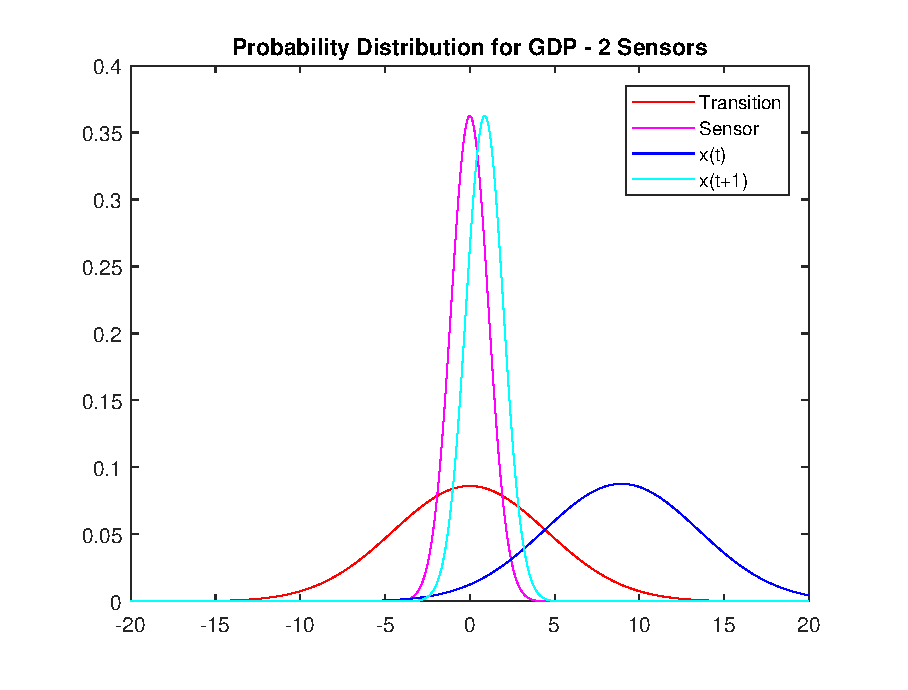
\includegraphics[width=10cm]{pd_1}
	
	\caption{Kalman Filter Related Probability Distribution}
	\label{fig:pd_1}
	
\end{figure}

\subsubsection{Extra Part: Additional Sensor for GDP growth rate }

The Kalman filter estimate for the GDP data is illustrated in figure~\ref{fig:kf2}.

\begin{figure}[htbp]
	
	\centering 
	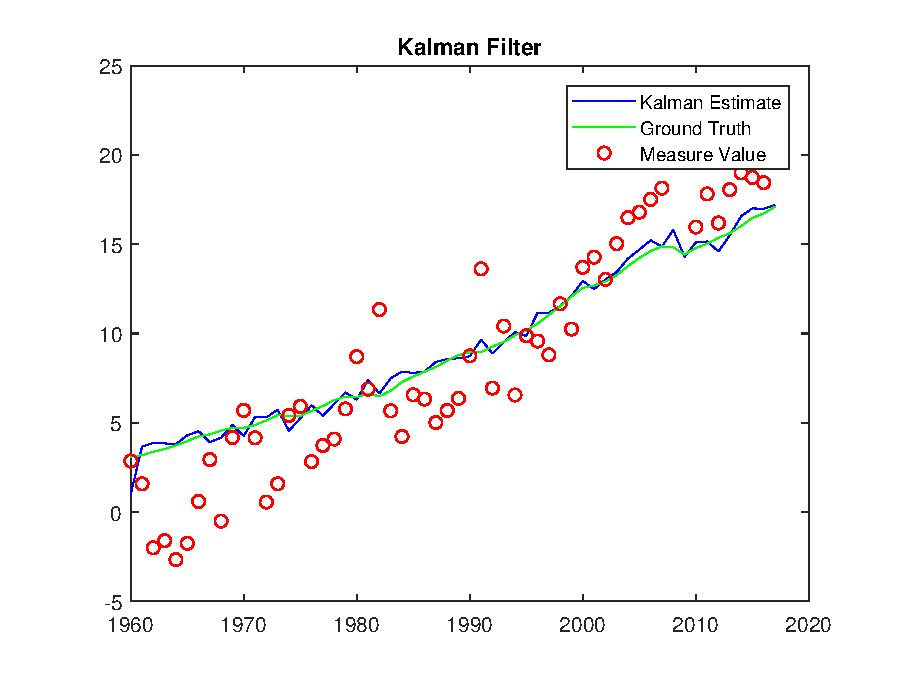
\includegraphics[width=10cm]{kf_2}
	
	\caption{Kalman Filter Estimate Result}
	\label{fig:kf2}
	
\end{figure}

The probability distribution is illustrated in~\ref{fig:pd_2}.

\begin{figure}[htbp]
	
	\centering 
	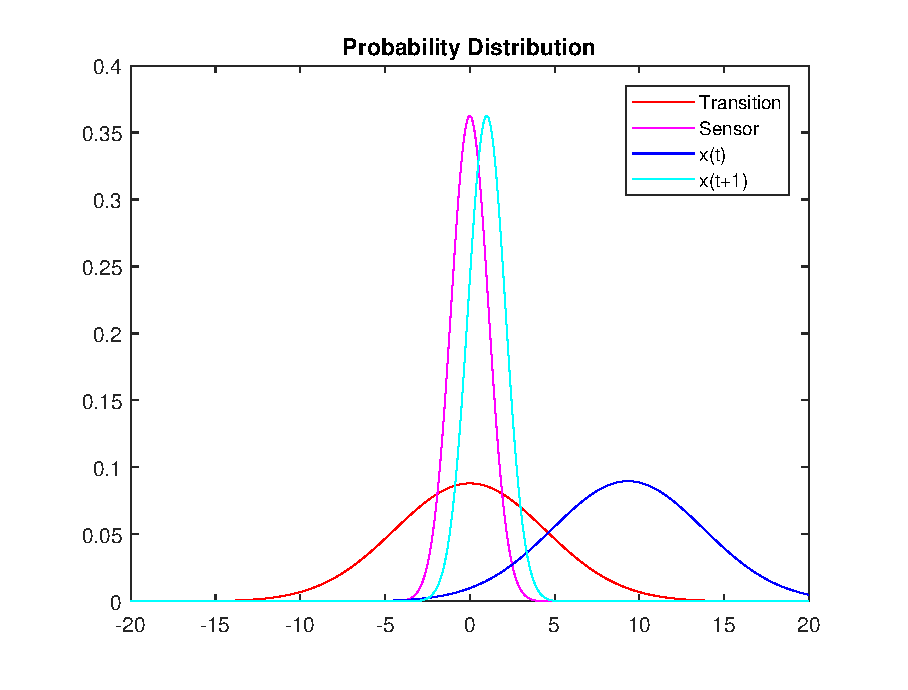
\includegraphics[width=10cm]{pd_2}
	
	\caption{Kalman Filter Related Probability Distribution}
	\label{fig:pd_2}
	
\end{figure}


\subsection{Discussion}

In the result part, the Kalman estimate result for the sensor model with 2 sensors and 3 sensors are given. In this part, we will use the Pearson's cofficient to compare the fitting result for the 2 sensors and 3 sensors.

\begin{table}[htbp] 
	\begin{center}
		\caption{Comparison}
		\begin{tabular}{l|l}  \hline
			Category & Value \\ \hline
			GDP Ground Truth Variance & 18.6672 \\ \hline
			2 Sensors Fitting Variance &  19.3499 \\ \hline
			3 Sensors Fitting Variance & 18.3853 \\ \hline
		\end{tabular}
		
		\label{tab:kf_meaning2}
	\end{center}
\end{table}	

The Pearson's coefficient table. The higher value means that the better fitting result.

\begin{table}[htbp] 
	\begin{center}
		\caption{Pearson's Coefficient}
		\begin{tabular}{l|l}  \hline
			Category & Value \\ \hline
			2 Sensors Fitting Variance & 0.9742 \\ \hline
			3 Sensors Fitting Variance & 0.9919 \\ \hline
		\end{tabular}
		
		\label{tab:kf_meaning3}
	\end{center}
\end{table}	

From table~\ref{tab:kf_meaning2} and~\ref*{tab:kf_meaning3}, the 3 sensor model illustrated a better fitting result, the variance deviation is smaller and the Pearson's coefficieint is higher.


\bibliographystyle{IEEEtran}  
\bibliography{MyRefs} 
%\addcontentsline{toc}{section}{References}





%-------------------------------------------------------------------------------------------------------





\end{document}
